\begin{center}
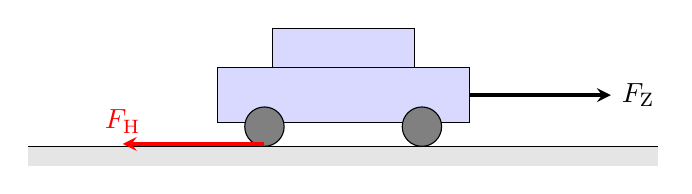
\begin{tikzpicture}[>=stealth]
 \fill[gray!20] (-4,0) rectangle (4,-0.25);
 \draw (-4,0) -- (4,0);
 \draw[fill=blue!15] (-1.6,0.3) rectangle (1.6,1.0);
 \draw[fill=blue!15] (-0.9,1.0) rectangle (0.9,1.5);
 \draw[fill=gray] (-1.0,0.25) circle (0.25) (1.0,0.25) circle (0.25);
 \draw[->, very thick] (1.6,0.65) -- ++(1.8,0) node[right] {$F_\mathrm{Z}$};
 \draw[->, very thick, red] (-1.0,0.03) -- ++(-1.8,0) node[above] {$F_\mathrm{H}$};
\end{tikzpicture}
\end{center}

Wir nehmen an, dass die blockierten Räder das ganze Gewicht tragen und das Auto auf trockenem Asphalt steht. Die Haftreibung hält das Auto, bis die Zugkraft die maximale Haftreibungskraft übersteigt. Mit $\mu_\mathrm{H} = \muHO$ für Pneu auf trockener Asphaltstrasse (FoTaBe S.~189) ist
\begin{align}
 F_\mathrm{Z} &> \FZuF \\
   &= \muH\cdot\mAu\cdot\gE \\
   &= \FZu \approx \result{\FZuP{3}{2}}
\end{align}
Bremst die Handbremse nur die Hinterräder, so tragen diese nur einen Teil des Gewichts, und die nötige Zugkraft ist entsprechend kleiner.
